\newpage
\chapter{Batch Reactor}

\section{Introduction}
The batch reactor model of Camflow has limited features. The limitation of the batch reactor models is that it is a constant volume batch reactor model and does not solve the energy equation. Only isothermal calculations can be performed with the batch reactor model of Camflow. 

\section{Fundamentals}
The following governing equation is solved
\begin{equation}
 \rho \frac{dY_k}{dt} = \dot{s}_k \bar{W}, \quad k=1\ldots K_g.
\end{equation}
Here $\rho$ is the density of the fluid, $Y_k$ is the mass fraction of the k\'th species, $\dot{s}_k$ is the molar production rate of the k\'th chemical species in mol/m$^3$, and $\bar{W}$ is the average molecular weight of the mixture in kg/mol.


\section{Input file}
A complete input file (camflow.xml) for a batch reactor simulation is shown below
{\scriptsize{
 \begin{verbatim}
<?xml version="1.0" encoding="ISO-8859-1"?>
<camflow>
   <reactor model="batch_cv">
   </reactor>
   <op_condition>
      <temperature>isothermal</temperature>	  
      <pressure unit="Pa">1e5</pressure>
   </op_condition>
   <inlet>
     <fuel>       
       <temperature unit="C">800</temperature>       
       <molefrac>
         <species name="NO2">0.1</species>
         <species name="N2">*</species>
       </molefrac>
     </fuel>
   </inlet>
   <solver mode="coupled" solver="cvode">
     <tols>
       <species>
         <aTol>1.e-10</aTol>
         <rTol>1.e-08</rTol>	  
       </species>
       <temperature>
         <aTol>1.e-03</aTol>
         <rTol>1.e-03</rTol>	  
       </temperature>
       <flow>
         <aTol>1.e-03</aTol>
         <rTol>1.e-03</rTol>	  
       </flow>
     </tols>
   </solver>
 <report species="mole">
 </report>
</camflow>

\end{verbatim}}
}
The input file follows xml specifications, with camflow as the root element and a number of child elements.
Each child element and its purpose is described below
\begin{itemize}
 \item \textbf{rector} : The reactor element specifies which reactor models is to be simulated and for a constant volume batch reactor camflow expects batch\_cv as the model attribute value.

\item \textbf{op\_conditions} : The element op\_conditions describes the operating conditions for the batch reactor. This includes the specification of the pressure and the condition applied to the solution of energy equation. Currently this model support only isothermal condition, and therefore temperature element should be assigned with isothermal condition.
\item \textbf{inlet} : The inlet element holds the information on reactants and the reactant temperature at time t=0. The temperature of the reactants must be specified using the temperature element with the appropriate units. The mass or mole fraction of the reactant species need to be specified within the element molefrac or massfrac. The sum of mass fractions or mole fraction of the reactant species must sum up to 1. Instead of specifying the mass/mole fractions of all species, the last species can be assigned with *. In this case the mole/mass fraction of the last species will be 1-sum of others.

\item \textbf{solver}: The solver element holds the solver control specifications. The attributes ``mode'' should always be specified as ``coupled'' for batch reactor simulation. The solver name is essentially provided to switch from one solver to another. However, the present version of Camflow uses only CVode as the numerical integrator, and therefore accepts only ``cvode'' as the solver name. The element tols hold the various tolarences that can be applied to the species, energy, and continuity equations. For species a relative tolarence of at least 10$^{-6}$ should be used. The user may need to adjust the tolarence values for the species in case of solution difficulties.

\item \textbf{report}: The desired output for the species composition must be specified in this element using the species attribute. ``mole'' or ``mass'' may be used as the attribute values, and correspondingly the output will be produced either in mole fraction or mass fractions.

\section{Executing the binary}
The batch reactor model of Camflow expects three input files namely, ``camflow.xml'', ``therm.dat'', and ``chem.inp''. All these files must be present in the working directory. Upon succesful execution the output file ``profile.dat'' containing the integration time(s), pressure (Pa), density (kg/m$^3$), temperature (K), and the species compositions in mass or mole fractions.
\end{itemize}

\section{Results}
The following figure shows the major species that results from the batch reactor model using ABF mechanism with a fuel composition of 50 \% O$_2$ and 50 \%C$_2$H$_4$
\begin{figure*}[h]
 \centering
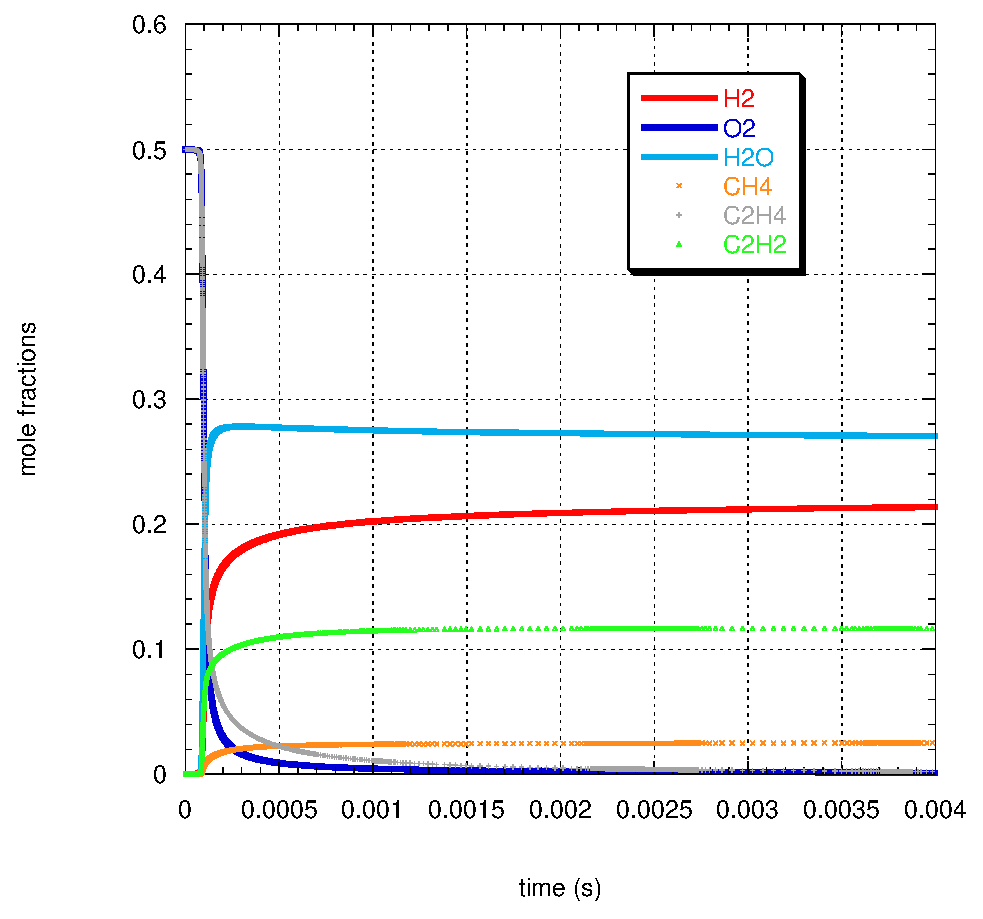
\includegraphics[scale=0.8]{batch_profile.eps}
\caption{Species profiles for ABF mechanism at isothermal condition of 1500 K}
\end{figure*}

%===============================================================================================
%
%
%
%===============================================================================================
